\documentclass[aspectratio=169]{beamer}

\usepackage{ccicons}
\usepackage{fontspec}
\usepackage{listings}
\usepackage{tikz}
\usepackage{svg}

\definecolor{uclablue}{RGB}{39,116,174}
\definecolor{uclagold}{RGB}{255,179,0}

\definecolor{ubcorange}{RGB}{158, 66, 37}

\definecolor{cugold}{RGB}{207, 184, 124}
\definecolor{cudarkgray}{RGB}{86, 90, 92}

\definecolor{solarizedred}{RGB}{220, 50, 47}
\definecolor{solarizedblue}{RGB}{38, 139, 210}
\definecolor{solarizedgreen}{RGB}{133, 153, 0}
\definecolor{solarizedpurple}{RGB}{108, 113, 196}
\definecolor{solarizedmagenta}{RGB}{211, 54, 130}

\definecolor{pantone655}{RGB}{0, 42, 92}
\definecolor{pantone7453}{RGB}{123, 164, 217}
\definecolor{pantone633}{RGB}{0, 139, 176}
\definecolor{pantone7492}{RGB}{218, 229, 205}

\colorlet{primarycolor}{pantone655}
\colorlet{secondarycolor}{pantone7453}


\usetikzlibrary{
  arrows,
  arrows.meta,
  automata,
  backgrounds,
  calc,
  chains,
  decorations.pathreplacing,
  fit,
  intersections,
  matrix,
  overlay-beamer-styles,
  positioning,
  shapes,
  shapes.multipart,
  tikzmark,
}
\usetikzmarklibrary{listings}

\hypersetup{
  colorlinks=true,
  urlcolor=cudarkgray,
}

\setbeamercolor{frametitle}{fg=primarycolor}
\setbeamercolor{structure}{fg=primarycolor}
\setbeamercolor{enumerate item}{fg=black}
\setbeamercolor{itemize item}{fg=black}
\setbeamercolor{itemize subitem}{fg=black}

\setbeamersize{text margin left=26.6mm}
\addtolength{\headsep}{2mm}

\setbeamertemplate{navigation symbols}{}
\setbeamertemplate{headline}{}
\setbeamertemplate{footline}{}
\setbeamertemplate{itemize item}{\color{black}}
\setbeamertemplate{itemize items}[circle]

\setbeamertemplate{footline}{
  \begin{tikzpicture}[remember picture,
                      overlay,
                      shift={(current page.south west)}]
    \node [black!50, inner sep=2mm, anchor=south east]
          at (current page.south east) {\footnotesize \insertframenumber};
  \end{tikzpicture}
}

\setsansfont{Inter}[Scale=MatchLowercase]
\setmonofont{Hack}[Scale=MatchLowercase]

\makeatletter
\newcommand\version[1]{\renewcommand\@version{#1}}
\newcommand\@version{}
\def\insertversion{\@version}

\newcommand\lecturenumber[1]{\renewcommand\@lecturenumber{#1}}
\newcommand\@lecturenumber{}
\def\insertlecturenumber{\@lecturenumber}
\makeatother

\setbeamertemplate{title page}
{
  \begin{tikzpicture}[remember picture,
                      overlay,
                      shift={(current page.south west)},
                      background rectangle/.style={fill=pantone655},
                      show background rectangle]
    \node [anchor=west, align=left, inner sep=0, text=white]
          (lecturenumber) at (\paperwidth / 6, \paperheight * 3 / 4)
          {\Large Lecture \insertlecturenumber};
    \node [inner sep=0, align=left, text=white, node distance=0,
          above left=of lecturenumber, anchor=south west, yshift=2mm]
          {\Large ECE 344: Operating Systems};
    \node (title) [inner sep=0, anchor=west, align=left, text=white,
                   text width=30em]
          at (\paperwidth / 6, \paperheight / 2)
          {{\bfseries \Huge \inserttitle{}}};
    \node [inner sep=0, align=right, text=white, node distance=0,
          below right=of title, anchor=north east, yshift=-1mm]
          {{\footnotesize \ttfamily \insertversion}};
    \node [inner sep=0, text=white, align=left, anchor=west]
          (author) at (\paperwidth / 6, \paperheight / 4)
          {\insertauthor};
    \node [text=white, inner sep=0, align=left, node distance=0,
           below left=of author, anchor=north west, yshift=-2mm]
          {\insertdate};
    \node [align=right, anchor=south east, inner sep=2mm, text=white]
          (license) at (\paperwidth, 0)
          {\footnotesize This  work is licensed under a
           \href{http://creativecommons.org/licenses/by-sa/4.0/}
                {\color{pantone7453} Creative Commons Attribution-ShareAlike 4.0
                 International License}};
    \node [text=white, inner sep=0, align=right, node distance=0,
           above right=of license, anchor=south east, xshift=-2mm]
          {\Large \ccbysa};
  \end{tikzpicture}
}

\tikzset{
  >=Straight Barb[],
  shorten >=1pt,
  initial text=,
}

\lstset{
  basicstyle=\footnotesize\ttfamily,
  language=C,
  escapechar=@,
  commentstyle=\color{black!50},
}


\lecturenumber{14}
\title{Basic Scheduling}
\version{1.0.0}
\author{Jon Eyolfson}
\date{October 11/12, 2022}

\begin{document}
  \begin{frame}[plain, noframenumbering]
    \titlepage
  \end{frame}

  \begin{frame}
    \frametitle{There are Preemptible and Non-preemptible Resources}

    A preemptible resource can be taken away and used for something else

    \hspace{2em} e.g. a CPU

    \vspace{2em}

    The resource is shared through scheduling

    \vspace{4em}

    A non-preemptible resource can not be taken away without acknowledgment

    \hspace{2em} e.g. disk space

    \vspace{2em}

    The resource is shared through allocations and deallocations

    \hspace{2em} Note: Parallel and distributed systems may allow you to allocate a CPU
  \end{frame}

  \begin{frame}
    \frametitle{A Dispatcher and Scheduler Work Together}

    A dispatcher is a low-level mechanism

    \hspace{2em} Responsible for context switching

    \vspace{2em}

    A scheduler is a high-level policy

    \hspace{2em} Responsible for deciding which processes to run
  \end{frame}

  \begin{frame}
    \frametitle{The Scheduler Runs Whenever a Process Changes State}

    First let's consider non-preemptable processes

    \hspace{2em} Once the process starts, it runs until completion

    \vspace{2em}

    In this case, the scheduler will only make a decision when the process
    terminates

    \vspace{4em}

    Preemptive allows the operating system to run the scheduler at will

    \hspace{2em} Check \texttt{uname -v}, your kernel should tell you it's preemptable
  \end{frame}

  \begin{frame}
    \frametitle{Metrics}

    Minimize waiting time and response time

    \hspace{2em} Don't have a process waiting too long (or too long to start)

    \vspace{2em}

    Maximize CPU utilization

    \hspace{2em} Don't have the CPU idle

    \vspace{2em}

    Maximize throughput

    \hspace{2em} Complete as many processes as possible

    \vspace{2em}

    Fairness

    \hspace{2em} Try to give each process the same percentage of the CPU
  \end{frame}

  \begin{frame}
    \frametitle{First Come First Served (FCFS)}

    The most basic form of scheduling

    \vspace{2em}

    The first process that arrives gets the CPU

    \vspace{2em}

    Processes are stored in a FIFO queue in arrival order
  \end{frame}
  
  \begin{frame}
    \frametitle{A Gantt Chart Illustrates the Schedule}

    Consider the following processes:
    \begin{center}
      \footnotesize
      \begin{tabular}{lrr}
        Process & Arrival Time & Burst Time \\
        $\mathsf{P_1}$ & 0 & 7 \\
        $\mathsf{P_2}$ & 0 & 4 \\
        $\mathsf{P_3}$ & 0 & 1 \\
        $\mathsf{P_4}$ & 0 & 4 \\
      \end{tabular}
    \end{center}

    Assume, $\mathsf{P_1} \rightarrow \mathsf{P_2} \rightarrow \mathsf{P_3}
             \rightarrow \mathsf{P_4}$.
    For FCFS, our schedule is:
    \begin{center}
      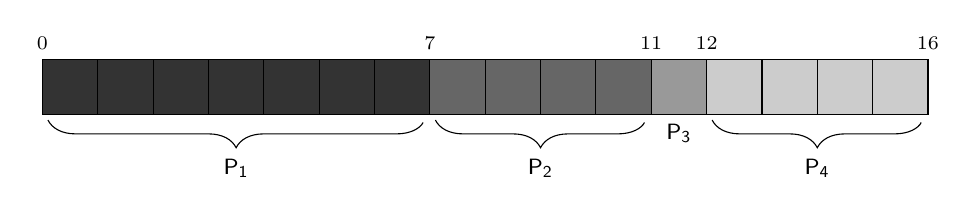
\begin{tikzpicture}

        \fill [black!80] (0,0) rectangle (14em, 2em);

        \fill [black!60] (14em,0) rectangle (22em, 2em);

        \fill [black!40] (22em,0) rectangle (24em, 2em);

        \fill [black!20] (24em,0) rectangle (32em, 2em);

        \draw (0,0) rectangle (32em,2em);

        \foreach \i in {1,...,15} {
          \draw [shorten >=0] (\i * 2em, 0) -- (\i * 2em, 2em);
        }

        \node [anchor=south] at (0em, 2em) {\scriptsize 0};
        \node [anchor=south] at (14em, 2em) {\scriptsize 7};
        \node [anchor=south] at (22em, 2em) {\scriptsize 11};
        \node [anchor=south] at (24em, 2em) {\scriptsize 12};
        \node [anchor=south] at (32em, 2em) {\scriptsize 16};

        \draw [decorate, decoration={brace,amplitude=10pt,mirror,raise=2pt}]
              (0.2em,0) -- (13.8em,0)
              node [midway, below, anchor=north, yshift=-1.25em]
              {\footnotesize $\mathsf{P_1}$};

        \draw [decorate, decoration={brace,amplitude=10pt,mirror,raise=2pt}]
              (14.2em,0) -- (21.8em,0)
              node [midway, below, anchor=north, yshift=-1.25em]
              {\footnotesize $\mathsf{P_2}$};

        \node [anchor=north] at (23em, 0) {\footnotesize $\mathsf{P_3}$};

        \draw [decorate, decoration={brace,amplitude=10pt,mirror,raise=2pt}]
              (24.2em,0) -- (31.8em,0)
              node [midway, below, anchor=north, yshift=-1.25em]
              {\footnotesize $\mathsf{P_4}$};
      \end{tikzpicture}
    \end{center}

    What is the average waiting time?
  \end{frame}
  
  \begin{frame}
    \frametitle{What Happens to Our Waiting Time with a Different Arrival Order}

    Consider the same processes:
    \begin{center}
      \footnotesize
      \begin{tabular}{lrr}
        Process & Arrival Time & Burst Time \\
        $\mathsf{P_1}$ & 0 & 7 \\
        $\mathsf{P_2}$ & 0 & 4 \\
        $\mathsf{P_3}$ & 0 & 1 \\
        $\mathsf{P_4}$ & 0 & 4 \\
      \end{tabular}
    \end{center}

    Assume, $\mathsf{P_3} \rightarrow \mathsf{P_2} \rightarrow \mathsf{P_4}
             \rightarrow \mathsf{P_1}$.
    For FCFS, our schedule is:
    \begin{center}
      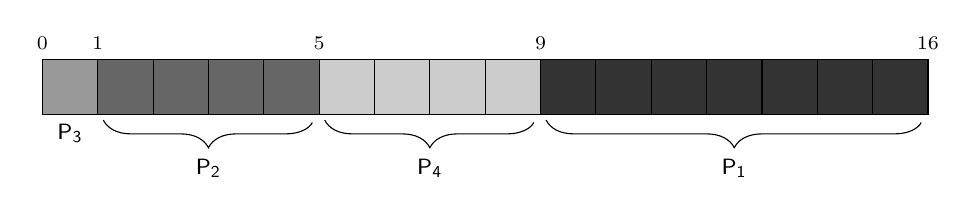
\begin{tikzpicture}

        \fill [black!80] (18em,0) rectangle (32em, 2em);

        \fill [black!60] (2em,0) rectangle (10em, 2em);

        \fill [black!40] (0em,0) rectangle (2em, 2em);

        \fill [black!20] (10em,0) rectangle (18em, 2em);

        \draw (0,0) rectangle (32em,2em);

        \foreach \i in {1,...,15} {
          \draw [shorten >=0] (\i * 2em, 0) -- (\i * 2em, 2em);
        }

        \node [anchor=south] at (0em, 2em) {\scriptsize 0};
        \node [anchor=south] at (2em, 2em) {\scriptsize 1};
        \node [anchor=south] at (10em, 2em) {\scriptsize 5};
        \node [anchor=south] at (18em, 2em) {\scriptsize 9};
        \node [anchor=south] at (32em, 2em) {\scriptsize 16};

        \node [anchor=north] at (1em, 0) {\footnotesize $\mathsf{P_3}$};

        \draw [decorate, decoration={brace,amplitude=10pt,mirror,raise=2pt}]
              (18.2em,0) -- (31.8em,0)
              node [midway, below, anchor=north, yshift=-1.25em]
              {\footnotesize $\mathsf{P_1}$};

        \draw [decorate, decoration={brace,amplitude=10pt,mirror,raise=2pt}]
              (2.2em,0) -- (9.8em,0)
              node [midway, below, anchor=north, yshift=-1.25em]
              {\footnotesize $\mathsf{P_2}$};

        \draw [decorate, decoration={brace,amplitude=10pt,mirror,raise=2pt}]
              (10.2em,0) -- (17.8em,0)
              node [midway, below, anchor=north, yshift=-1.25em]
              {\footnotesize $\mathsf{P_4}$};
      \end{tikzpicture}
    \end{center}

    What is the average waiting time now?
  \end{frame}

  \begin{frame}
    \frametitle{Shortest Job First (SJF)}

    A slight tweak to FCFS, we always schedule the job with the shortest burst time
    first

    \vspace{2em}

    We're still assuming no preemption
  \end{frame}

  \begin{frame}
    \frametitle{SJF Minimizes the Average Wait Time over FCFS}

    Consider the same processes with different arrival times:
    \begin{center}
      \footnotesize
      \begin{tabular}{lrr}
        Process & Arrival Time & Burst Time \\
        $\mathsf{P_1}$ & 0 & 7 \\
        $\mathsf{P_2}$ & 2 & 4 \\
        $\mathsf{P_3}$ & 4 & 1 \\
        $\mathsf{P_4}$ & 5 & 4 \\
      \end{tabular}
    \end{center}

    For SJF, our schedule is (arrival on top):
    \begin{center}
      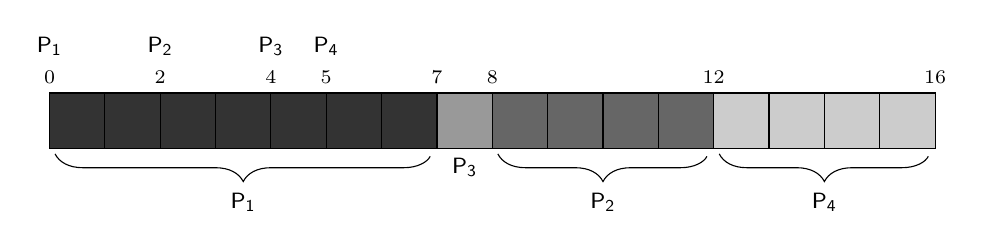
\begin{tikzpicture}

        \fill [black!80] (0,0) rectangle (14em, 2em);

        \fill [black!60] (16em,0) rectangle (24em, 2em);

        \fill [black!40] (14em,0) rectangle (16em, 2em);

        \fill [black!20] (24em,0) rectangle (32em, 2em);

        \draw (0,0) rectangle (32em,2em);

        \foreach \i in {1,...,15} {
          \draw [shorten >=0] (\i * 2em, 0) -- (\i * 2em, 2em);
        }

        \node [anchor=south] at (0em, 2em) {\scriptsize 0};
        \node [anchor=south] at (4em, 2em) {\scriptsize 2};
        \node [anchor=south] at (8em, 2em) {\scriptsize 4};
        \node [anchor=south] at (10em, 2em) {\scriptsize 5};
        \node [anchor=south] at (14em, 2em) {\scriptsize 7};
        \node [anchor=south] at (16em, 2em) {\scriptsize 8};
        \node [anchor=south] at (24em, 2em) {\scriptsize 12};
        \node [anchor=south] at (32em, 2em) {\scriptsize 16};

        \draw [decorate, decoration={brace,amplitude=10pt,mirror,raise=2pt}]
              (0.2em,0) -- (13.8em,0)
              node [midway, below, anchor=north, yshift=-1.25em]
              {\footnotesize $\mathsf{P_1}$};

        \draw [decorate, decoration={brace,amplitude=10pt,mirror,raise=2pt}]
              (16.2em,0) -- (23.8em,0)
              node [midway, below, anchor=north, yshift=-1.25em]
              {\footnotesize $\mathsf{P_2}$};

        \node [anchor=north] at (15em, 0) {\footnotesize $\mathsf{P_3}$};

        \draw [decorate, decoration={brace,amplitude=10pt,mirror,raise=2pt}]
              (24.2em,0) -- (31.8em,0)
              node [midway, below, anchor=north, yshift=-1.25em]
              {\footnotesize $\mathsf{P_4}$};

        \node [anchor=south, yshift=1em] at (0em, 2em) {\footnotesize $\mathsf{P_1}$};

        \node [anchor=south, yshift=1em] at (4em, 2em) {\footnotesize $\mathsf{P_2}$};

        \node [anchor=south, yshift=1em] at (8em, 2em) {\footnotesize $\mathsf{P_3}$};

        \node [anchor=south, yshift=1em] at (10em, 2em) {\footnotesize $\mathsf{P_4}$};
      \end{tikzpicture}
    \end{center}

    Average waiting time: $\mathsf{\frac{0 + 6 + 3 + 7}{4} = 4}$
  \end{frame}

  \begin{frame}
    \frametitle{SJF is Not Practical}

    It is provably optimal at minimizing average wait time (if no preemption)

    \vspace{2em}

    You will not know the burst times of each process

    \hspace{2em} You could use the past to predict future executions

    \vspace{2em}

    You may starve long jobs (they may never execute)
  \end{frame}

  \begin{frame}
    \frametitle{Shortest Remaining Time First (SRTF)}

    Changing SJF to run with preemptions requires another tweak

    \vspace{2em}

    We'll assume that our minimum execution time is one unit

    \vspace{2em}

    Similar to SJF, this optimizes the average waiting time
  \end{frame}

  \begin{frame}
    \frametitle{SRTF Reduces the Average Wait Time Compared to SJF}

    Consider the same processes and arrival times as SJF:
    \begin{center}
      \footnotesize
      \begin{tabular}{lrr}
        Process & Arrival Time & Burst Time \\
        $\mathsf{P_1}$ & 0 & 7 \\
        $\mathsf{P_2}$ & 2 & 4 \\
        $\mathsf{P_3}$ & 4 & 1 \\
        $\mathsf{P_4}$ & 5 & 4 \\
      \end{tabular}
    \end{center}

    For SRTF, our schedule is (arrival on top):
    \begin{center}
      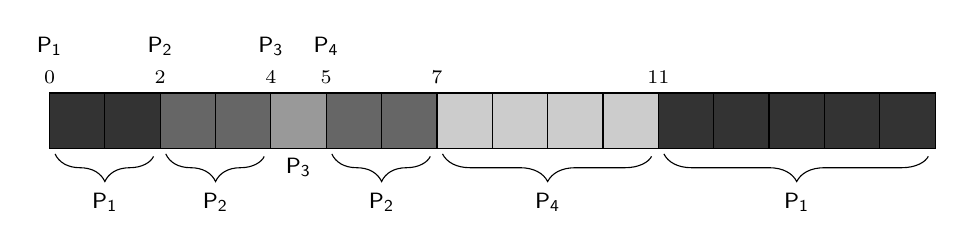
\begin{tikzpicture}

        \fill [black!80] (0,0) rectangle (4em, 2em);

        \fill [black!60] (4em,0) rectangle (8em, 2em);

        \fill [black!40] (8em,0) rectangle (10em, 2em);

        \fill [black!60] (10em,0) rectangle (14em, 2em);

        \fill [black!20] (14em,0) rectangle (22em, 2em);

        \fill [black!80] (22em,0) rectangle (32em, 2em);

        \draw (0,0) rectangle (32em,2em);

        \foreach \i in {1,...,15} {
          \draw [shorten >=0] (\i * 2em, 0) -- (\i * 2em, 2em);
        }

        \node [anchor=south] at (0em, 2em) {\scriptsize 0};
        \node [anchor=south] at (4em, 2em) {\scriptsize 2};
        \node [anchor=south] at (8em, 2em) {\scriptsize 4};
        \node [anchor=south] at (10em, 2em) {\scriptsize 5};
        \node [anchor=south] at (14em, 2em) {\scriptsize 7};
        \node [anchor=south] at (22em, 2em) {\scriptsize 11};

        \draw [decorate, decoration={brace,amplitude=10pt,mirror,raise=2pt}]
              (0.2em,0) -- (3.8em,0)
              node [midway, below, anchor=north, yshift=-1.25em]
              {\footnotesize $\mathsf{P_1}$};

        \draw [decorate, decoration={brace,amplitude=10pt,mirror,raise=2pt}]
              (4.2em,0) -- (7.8em,0)
              node [midway, below, anchor=north, yshift=-1.25em]
              {\footnotesize $\mathsf{P_2}$};

        \node [anchor=north] at (9em, 0) {\footnotesize $\mathsf{P_3}$};

        \draw [decorate, decoration={brace,amplitude=10pt,mirror,raise=2pt}]
              (10.2em,0) -- (13.8em,0)
              node [midway, below, anchor=north, yshift=-1.25em]
              {\footnotesize $\mathsf{P_2}$};

        \draw [decorate, decoration={brace,amplitude=10pt,mirror,raise=2pt}]
              (14.2em,0) -- (21.8em,0)
              node [midway, below, anchor=north, yshift=-1.25em]
              {\footnotesize $\mathsf{P_4}$};
              
        \draw [decorate, decoration={brace,amplitude=10pt,mirror,raise=2pt}]
              (22.2em,0) -- (31.8em,0)
              node [midway, below, anchor=north, yshift=-1.25em]
              {\footnotesize $\mathsf{P_1}$};

        \node [anchor=south, yshift=1em] at (0em, 2em) {\footnotesize $\mathsf{P_1}$};

        \node [anchor=south, yshift=1em] at (4em, 2em) {\footnotesize $\mathsf{P_2}$};

        \node [anchor=south, yshift=1em] at (8em, 2em) {\footnotesize $\mathsf{P_3}$};

        \node [anchor=south, yshift=1em] at (10em, 2em) {\footnotesize $\mathsf{P_4}$};
      \end{tikzpicture}
    \end{center}

    Average waiting time: $\mathsf{\frac{9 + 1 + 0 + 2}{4} = 3}$
  \end{frame}

  \begin{frame}
    \frametitle{Round-Robin (RR)}

    So far we haven't handled fairness (it's a trade off with other metrics)

    \vspace{2em}

    The operating system divides execution into time slices (or quanta)

    \hspace{2em} An individual time slice is called a quantum

    \vspace{2em}

    Maintain a FIFO queue of processes similar to FCFS

    \hspace{2em} Preempt if still running at end of quantum and re-add to queue

    \vspace{2em}

    What are practical considerations for determining quantum length?
  \end{frame}

  \begin{frame}
    \frametitle{RR with a Quantum Length of 3 Units}

    \begin{center}
      \footnotesize
      \begin{tabular}{lrr}
        Process & Arrival Time & Burst Time \\
        $\mathsf{P_1}$ & 0 & 7 \\
        $\mathsf{P_2}$ & 2 & 4 \\
        $\mathsf{P_3}$ & 4 & 1 \\
        $\mathsf{P_4}$ & 5 & 4 \\
      \end{tabular}
    \end{center}

    For RR, our schedule is (arrival on top, queue on bottom):
    \begin{center}
      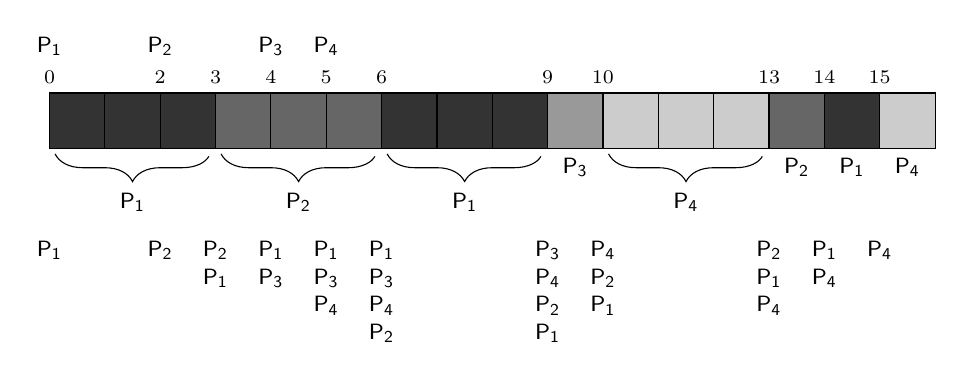
\begin{tikzpicture}

        \fill [black!80] (0,0) rectangle (6em, 2em);
        
        \fill [black!60] (6em,0) rectangle (12em, 2em);

        \fill [black!80] (12em,0) rectangle (18em, 2em);

        \fill [black!40] (18em,0) rectangle (20em, 2em);

        \fill [black!20] (20em,0) rectangle (26em, 2em);

        \fill [black!60] (26em,0) rectangle (28em, 2em);

        \fill [black!80] (28em,0) rectangle (30em, 2em);

        \fill [black!20] (30em,0) rectangle (32em, 2em);

        \draw (0,0) rectangle (32em,2em);

        \foreach \i in {1,...,15} {
          \draw [shorten >=0] (\i * 2em, 0) -- (\i * 2em, 2em);
        }

        \node [anchor=south] at (0em, 2em) {\scriptsize 0};
        \node [anchor=south] at (4em, 2em) {\scriptsize 2};
        \node [anchor=south] at (6em, 2em) {\scriptsize 3};
        \node [anchor=south] at (8em, 2em) {\scriptsize 4};
        \node [anchor=south] at (10em, 2em) {\scriptsize 5};
        \node [anchor=south] at (12em, 2em) {\scriptsize 6};
        \node [anchor=south] at (18em, 2em) {\scriptsize 9};
        \node [anchor=south] at (20em, 2em) {\scriptsize 10};
        \node [anchor=south] at (26em, 2em) {\scriptsize 13};
        \node [anchor=south] at (28em, 2em) {\scriptsize 14};
        \node [anchor=south] at (30em, 2em) {\scriptsize 15};

        \draw [decorate, decoration={brace,amplitude=10pt,mirror,raise=2pt}]
              (0.2em,0) -- (5.8em,0)
              node [midway, below, anchor=north, yshift=-1.25em]
              {\footnotesize $\mathsf{P_1}$};

        \draw [decorate, decoration={brace,amplitude=10pt,mirror,raise=2pt}]
              (6.2em,0) -- (11.8em,0)
              node [midway, below, anchor=north, yshift=-1.25em]
              {\footnotesize $\mathsf{P_2}$};

        \draw [decorate, decoration={brace,amplitude=10pt,mirror,raise=2pt}]
              (12.2em,0) -- (17.8em,0)
              node [midway, below, anchor=north, yshift=-1.25em]
              {\footnotesize $\mathsf{P_1}$};

        \node [anchor=north] at (19em, 0) {\footnotesize $\mathsf{P_3}$};

        \draw [decorate, decoration={brace,amplitude=10pt,mirror,raise=2pt}]
              (20.2em,0) -- (25.8em,0)
              node [midway, below, anchor=north, yshift=-1.25em]
              {\footnotesize $\mathsf{P_4}$};

        \node [anchor=north] at (27em, 0) {\footnotesize $\mathsf{P_2}$};

        \node [anchor=north] at (29em, 0) {\footnotesize $\mathsf{P_1}$};

        \node [anchor=north] at (31em, 0) {\footnotesize $\mathsf{P_4}$};

        \node [anchor=south, yshift=1em] at (0em, 2em) {\footnotesize $\mathsf{P_1}$};

        \node [anchor=south, yshift=1em] at (4em, 2em) {\footnotesize $\mathsf{P_2}$};

        \node [anchor=south, yshift=1em] at (8em, 2em) {\footnotesize $\mathsf{P_3}$};

        \node [anchor=south, yshift=1em] at (10em, 2em) {\footnotesize $\mathsf{P_4}$};

        \node [anchor=north, yshift=-3em] at (0em, 0em) {\footnotesize $\mathsf{P_1}$};

        \node [anchor=north, yshift=-3em] at (4em, 0em) {\footnotesize $\mathsf{P_2}$};

        \node [anchor=north, yshift=-3em] at (6em, 0em) {\footnotesize $\mathsf{P_2}$};
        \node [anchor=north, yshift=-4em] at (6em, 0em) {\footnotesize $\mathsf{P_1}$};

        \node [anchor=north, yshift=-3em] at (8em, 0em) {\footnotesize $\mathsf{P_1}$};
        \node [anchor=north, yshift=-4em] at (8em, 0em) {\footnotesize $\mathsf{P_3}$};

        \node [anchor=north, yshift=-3em] at (10em, 0em) {\footnotesize $\mathsf{P_1}$};
        \node [anchor=north, yshift=-4em] at (10em, 0em) {\footnotesize $\mathsf{P_3}$};
        \node [anchor=north, yshift=-5em] at (10em, 0em) {\footnotesize $\mathsf{P_4}$};

        \node [anchor=north, yshift=-3em] at (12em, 0em) {\footnotesize $\mathsf{P_1}$};
        \node [anchor=north, yshift=-4em] at (12em, 0em) {\footnotesize $\mathsf{P_3}$};
        \node [anchor=north, yshift=-5em] at (12em, 0em) {\footnotesize $\mathsf{P_4}$};
        \node [anchor=north, yshift=-6em] at (12em, 0em) {\footnotesize $\mathsf{P_2}$};

        \node [anchor=north, yshift=-3em] at (18em, 0em) {\footnotesize $\mathsf{P_3}$};
        \node [anchor=north, yshift=-4em] at (18em, 0em) {\footnotesize $\mathsf{P_4}$};
        \node [anchor=north, yshift=-5em] at (18em, 0em) {\footnotesize $\mathsf{P_2}$};
        \node [anchor=north, yshift=-6em] at (18em, 0em) {\footnotesize $\mathsf{P_1}$};

        \node [anchor=north, yshift=-3em] at (20em, 0em) {\footnotesize $\mathsf{P_4}$};
        \node [anchor=north, yshift=-4em] at (20em, 0em) {\footnotesize $\mathsf{P_2}$};
        \node [anchor=north, yshift=-5em] at (20em, 0em) {\footnotesize $\mathsf{P_1}$};

        \node [anchor=north, yshift=-3em] at (26em, 0em) {\footnotesize $\mathsf{P_2}$};
        \node [anchor=north, yshift=-4em] at (26em, 0em) {\footnotesize $\mathsf{P_1}$};
        \node [anchor=north, yshift=-5em] at (26em, 0em) {\footnotesize $\mathsf{P_4}$};

        \node [anchor=north, yshift=-3em] at (28em, 0em) {\footnotesize $\mathsf{P_1}$};
        \node [anchor=north, yshift=-4em] at (28em, 0em) {\footnotesize $\mathsf{P_4}$};

        \node [anchor=north, yshift=-3em] at (30em, 0em) {\footnotesize $\mathsf{P_4}$};
      \end{tikzpicture}
    \end{center}
  \end{frame}

  \begin{frame}
    \frametitle{Metrics for RR (3 Unit Quantum Length)}

    Number of context switches: 7

    \vspace{2em}

    Average waiting time: $\mathsf{\frac{8 + 8 + 5 + 7}{4} = 7}$

    \vspace{2em}

    Average response time: $\mathsf{\frac{0 + 1 + 5 + 5}{4} = 2.75}$

    \vspace{4em}

    Note: on ties (a new process arrives while one is preempted), favor the new one
  \end{frame}

  \begin{frame}
    \frametitle{RR with a Quantum Length of 1 Units}

    \begin{center}
      \footnotesize
      \begin{tabular}{lrr}
        Process & Arrival Time & Burst Time \\
        $\mathsf{P_1}$ & 0 & 7 \\
        $\mathsf{P_2}$ & 2 & 4 \\
        $\mathsf{P_3}$ & 4 & 1 \\
        $\mathsf{P_4}$ & 5 & 4 \\
      \end{tabular}
    \end{center}

    For RR, our schedule is (arrival on top, queue on bottom):
    \begin{center}
      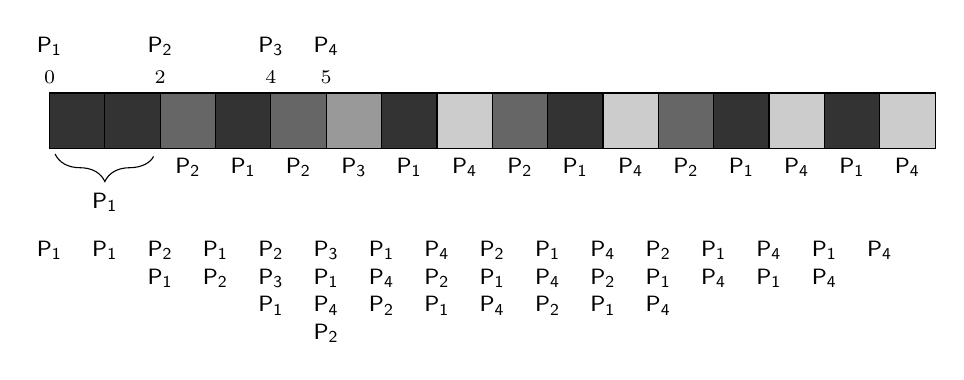
\begin{tikzpicture}

        \fill [black!80] (0,0) rectangle (4em, 2em);
        \fill [black!60] (4em,0) rectangle (6em, 2em);
        \fill [black!80] (6em,0) rectangle (8em, 2em);
        \fill [black!60] (8em,0) rectangle (10em, 2em);
        \fill [black!40] (10em,0) rectangle (12em, 2em);
        \fill [black!80] (12em,0) rectangle (14em, 2em);
        \fill [black!20] (14em,0) rectangle (16em, 2em);
        \fill [black!60] (16em,0) rectangle (18em, 2em);
        \fill [black!80] (18em,0) rectangle (20em, 2em);
        \fill [black!20] (20em,0) rectangle (22em, 2em);
        \fill [black!60] (22em,0) rectangle (24em, 2em);
        \fill [black!80] (24em,0) rectangle (26em, 2em);
        \fill [black!20] (26em,0) rectangle (28em, 2em);
        \fill [black!80] (28em,0) rectangle (30em, 2em);
        \fill [black!20] (30em,0) rectangle (32em, 2em);

        \draw (0,0) rectangle (32em,2em);

        \foreach \i in {1,...,15} {
          \draw [shorten >=0] (\i * 2em, 0) -- (\i * 2em, 2em);
        }

        \node [anchor=south] at (0em, 2em) {\scriptsize 0};
        \node [anchor=south] at (4em, 2em) {\scriptsize 2};
        \node [anchor=south] at (8em, 2em) {\scriptsize 4};
        \node [anchor=south] at (10em, 2em) {\scriptsize 5};

        \draw [decorate, decoration={brace,amplitude=10pt,mirror,raise=2pt}]
              (0.2em,0) -- (3.8em,0)
              node [midway, below, anchor=north, yshift=-1.25em]
              {\footnotesize $\mathsf{P_1}$};

        \node [anchor=north] at (5em, 0) {\footnotesize $\mathsf{P_2}$};
        \node [anchor=north] at (7em, 0) {\footnotesize $\mathsf{P_1}$};
        \node [anchor=north] at (9em, 0) {\footnotesize $\mathsf{P_2}$};
        \node [anchor=north] at (11em, 0) {\footnotesize $\mathsf{P_3}$};
        \node [anchor=north] at (13em, 0) {\footnotesize $\mathsf{P_1}$};
        \node [anchor=north] at (15em, 0) {\footnotesize $\mathsf{P_4}$};
        \node [anchor=north] at (17em, 0) {\footnotesize $\mathsf{P_2}$};
        \node [anchor=north] at (19em, 0) {\footnotesize $\mathsf{P_1}$};
        \node [anchor=north] at (21em, 0) {\footnotesize $\mathsf{P_4}$};
        \node [anchor=north] at (23em, 0) {\footnotesize $\mathsf{P_2}$};
        \node [anchor=north] at (25em, 0) {\footnotesize $\mathsf{P_1}$};
        \node [anchor=north] at (27em, 0) {\footnotesize $\mathsf{P_4}$};
        \node [anchor=north] at (29em, 0) {\footnotesize $\mathsf{P_1}$};
        \node [anchor=north] at (31em, 0) {\footnotesize $\mathsf{P_4}$};

        % Arrivals
        \node [anchor=south, yshift=1em] at (0em, 2em) {\footnotesize $\mathsf{P_1}$};
        \node [anchor=south, yshift=1em] at (4em, 2em) {\footnotesize $\mathsf{P_2}$};
        \node [anchor=south, yshift=1em] at (8em, 2em) {\footnotesize $\mathsf{P_3}$};
        \node [anchor=south, yshift=1em] at (10em, 2em) {\footnotesize $\mathsf{P_4}$};

        % Queues
        \node [anchor=north, yshift=-3em] at (0em, 0em) {\footnotesize $\mathsf{P_1}$};

        \node [anchor=north, yshift=-3em] at (2em, 0em) {\footnotesize $\mathsf{P_1}$};

        \node [anchor=north, yshift=-3em] at (4em, 0em) {\footnotesize $\mathsf{P_2}$};
        \node [anchor=north, yshift=-4em] at (4em, 0em) {\footnotesize $\mathsf{P_1}$};

        \node [anchor=north, yshift=-3em] at (6em, 0em) {\footnotesize $\mathsf{P_1}$};
        \node [anchor=north, yshift=-4em] at (6em, 0em) {\footnotesize $\mathsf{P_2}$};

        \node [anchor=north, yshift=-3em] at (8em, 0em) {\footnotesize $\mathsf{P_2}$};
        \node [anchor=north, yshift=-4em] at (8em, 0em) {\footnotesize $\mathsf{P_3}$};
        \node [anchor=north, yshift=-5em] at (8em, 0em) {\footnotesize $\mathsf{P_1}$};

        \node [anchor=north, yshift=-3em] at (10em, 0em) {\footnotesize $\mathsf{P_3}$};
        \node [anchor=north, yshift=-4em] at (10em, 0em) {\footnotesize $\mathsf{P_1}$};
        \node [anchor=north, yshift=-5em] at (10em, 0em) {\footnotesize $\mathsf{P_4}$};
        \node [anchor=north, yshift=-6em] at (10em, 0em) {\footnotesize $\mathsf{P_2}$};

        \node [anchor=north, yshift=-3em] at (12em, 0em) {\footnotesize $\mathsf{P_1}$};
        \node [anchor=north, yshift=-4em] at (12em, 0em) {\footnotesize $\mathsf{P_4}$};
        \node [anchor=north, yshift=-5em] at (12em, 0em) {\footnotesize $\mathsf{P_2}$};

        \node [anchor=north, yshift=-3em] at (14em, 0em) {\footnotesize $\mathsf{P_4}$};
        \node [anchor=north, yshift=-4em] at (14em, 0em) {\footnotesize $\mathsf{P_2}$};
        \node [anchor=north, yshift=-5em] at (14em, 0em) {\footnotesize $\mathsf{P_1}$};

        \node [anchor=north, yshift=-3em] at (16em, 0em) {\footnotesize $\mathsf{P_2}$};
        \node [anchor=north, yshift=-4em] at (16em, 0em) {\footnotesize $\mathsf{P_1}$};
        \node [anchor=north, yshift=-5em] at (16em, 0em) {\footnotesize $\mathsf{P_4}$};

        \node [anchor=north, yshift=-3em] at (18em, 0em) {\footnotesize $\mathsf{P_1}$};
        \node [anchor=north, yshift=-4em] at (18em, 0em) {\footnotesize $\mathsf{P_4}$};
        \node [anchor=north, yshift=-5em] at (18em, 0em) {\footnotesize $\mathsf{P_2}$};

        \node [anchor=north, yshift=-3em] at (20em, 0em) {\footnotesize $\mathsf{P_4}$};
        \node [anchor=north, yshift=-4em] at (20em, 0em) {\footnotesize $\mathsf{P_2}$};
        \node [anchor=north, yshift=-5em] at (20em, 0em) {\footnotesize $\mathsf{P_1}$};

        \node [anchor=north, yshift=-3em] at (22em, 0em) {\footnotesize $\mathsf{P_2}$};
        \node [anchor=north, yshift=-4em] at (22em, 0em) {\footnotesize $\mathsf{P_1}$};
        \node [anchor=north, yshift=-5em] at (22em, 0em) {\footnotesize $\mathsf{P_4}$};

        \node [anchor=north, yshift=-3em] at (24em, 0em) {\footnotesize $\mathsf{P_1}$};
        \node [anchor=north, yshift=-4em] at (24em, 0em) {\footnotesize $\mathsf{P_4}$};

        \node [anchor=north, yshift=-3em] at (26em, 0em) {\footnotesize $\mathsf{P_4}$};
        \node [anchor=north, yshift=-4em] at (26em, 0em) {\footnotesize $\mathsf{P_1}$};

        \node [anchor=north, yshift=-3em] at (28em, 0em) {\footnotesize $\mathsf{P_1}$};
        \node [anchor=north, yshift=-4em] at (28em, 0em) {\footnotesize $\mathsf{P_4}$};

        \node [anchor=north, yshift=-3em] at (30em, 0em) {\footnotesize $\mathsf{P_4}$};
      \end{tikzpicture}
    \end{center}
  \end{frame}

  \begin{frame}
    \frametitle{Metrics for RR (1 Unit Quantum Length)}

    Number of context switches: 14

    \vspace{2em}

    Average waiting time: $\mathsf{\frac{8 + 6 + 1 + 7}{4} = 5.5}$

    \vspace{2em}

    Average response time: $\mathsf{\frac{0 + 0 + 1 + 2}{4} = 0.75}$
  \end{frame}

  \begin{frame}
    \frametitle{RR with a Quantum Length of 10 Units}

    \begin{center}
      \footnotesize
      \begin{tabular}{lrr}
        Process & Arrival Time & Burst Time \\
        $\mathsf{P_1}$ & 0 & 7 \\
        $\mathsf{P_2}$ & 2 & 4 \\
        $\mathsf{P_3}$ & 4 & 1 \\
        $\mathsf{P_4}$ & 5 & 4 \\
      \end{tabular}
    \end{center}

    For RR, our schedule is (arrival on top, queue on bottom):

    \begin{center}
      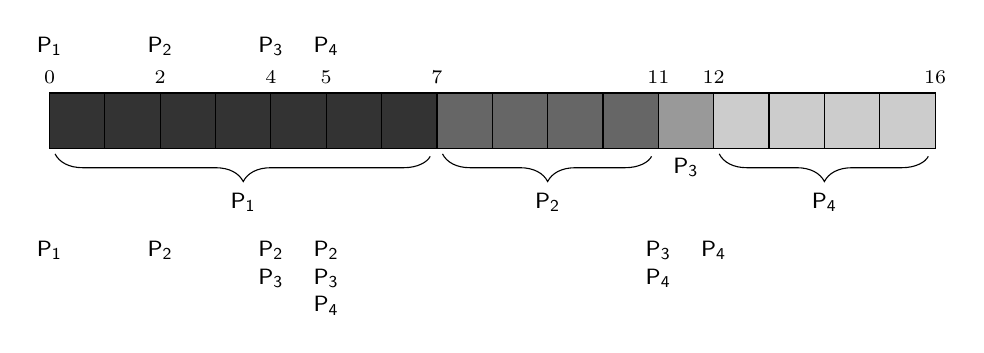
\begin{tikzpicture}

        \fill [black!80] (0,0) rectangle (14em, 2em);

        \fill [black!60] (14em,0) rectangle (22em, 2em);

        \fill [black!40] (22em,0) rectangle (24em, 2em);

        \fill [black!20] (24em,0) rectangle (32em, 2em);

        \draw (0,0) rectangle (32em,2em);

        \foreach \i in {1,...,15} {
          \draw [shorten >=0] (\i * 2em, 0) -- (\i * 2em, 2em);
        }

        \node [anchor=south] at (0em, 2em) {\scriptsize 0};
        \node [anchor=south] at (4em, 2em) {\scriptsize 2};
        \node [anchor=south] at (8em, 2em) {\scriptsize 4};
        \node [anchor=south] at (10em, 2em) {\scriptsize 5};
        \node [anchor=south] at (14em, 2em) {\scriptsize 7};
        \node [anchor=south] at (22em, 2em) {\scriptsize 11};
        \node [anchor=south] at (24em, 2em) {\scriptsize 12};
        \node [anchor=south] at (32em, 2em) {\scriptsize 16};

        % Arrivals
        \node [anchor=south, yshift=1em] at (0em, 2em) {\footnotesize $\mathsf{P_1}$};
        \node [anchor=south, yshift=1em] at (4em, 2em) {\footnotesize $\mathsf{P_2}$};
        \node [anchor=south, yshift=1em] at (8em, 2em) {\footnotesize $\mathsf{P_3}$};
        \node [anchor=south, yshift=1em] at (10em, 2em) {\footnotesize $\mathsf{P_4}$};

        % Queues
        \node [anchor=north, yshift=-3em] at (0em, 0em) {\footnotesize $\mathsf{P_1}$};

        \node [anchor=north, yshift=-3em] at (4em, 0em) {\footnotesize $\mathsf{P_2}$};

        \node [anchor=north, yshift=-3em] at (8em, 0em) {\footnotesize $\mathsf{P_2}$};
        \node [anchor=north, yshift=-4em] at (8em, 0em) {\footnotesize $\mathsf{P_3}$};

        \node [anchor=north, yshift=-3em] at (10em, 0em) {\footnotesize $\mathsf{P_2}$};
        \node [anchor=north, yshift=-4em] at (10em, 0em) {\footnotesize $\mathsf{P_3}$};
        \node [anchor=north, yshift=-5em] at (10em, 0em) {\footnotesize $\mathsf{P_4}$};

        \node [anchor=north, yshift=-3em] at (22em, 0em) {\footnotesize $\mathsf{P_3}$};
        \node [anchor=north, yshift=-4em] at (22em, 0em) {\footnotesize $\mathsf{P_4}$};

        \node [anchor=north, yshift=-3em] at (24em, 0em) {\footnotesize $\mathsf{P_4}$};


        \draw [decorate, decoration={brace,amplitude=10pt,mirror,raise=2pt}]
              (0.2em,0) -- (13.8em,0)
              node [midway, below, anchor=north, yshift=-1.25em]
              {\footnotesize $\mathsf{P_1}$};

        \draw [decorate, decoration={brace,amplitude=10pt,mirror,raise=2pt}]
              (14.2em,0) -- (21.8em,0)
              node [midway, below, anchor=north, yshift=-1.25em]
              {\footnotesize $\mathsf{P_2}$};

        \node [anchor=north] at (23em, 0) {\footnotesize $\mathsf{P_3}$};

        \draw [decorate, decoration={brace,amplitude=10pt,mirror,raise=2pt}]
              (24.2em,0) -- (31.8em,0)
              node [midway, below, anchor=north, yshift=-1.25em]
              {\footnotesize $\mathsf{P_4}$};
      \end{tikzpicture}
    \end{center}
  \end{frame}

  \begin{frame}
    \frametitle{Metrics for RR (10 Unit Quantum Length)}

    Number of context switches: 3

    \vspace{2em}

    Average waiting time: $\mathsf{\frac{0 + 5 + 7 + 7}{4} = 4.75}$

    \vspace{2em}

    Average response time: $\mathsf{\frac{0 + 5 + 7 + 7}{4} = 4.75}$

    \vspace{4em}

    Note: in this case it's the same as FCFS without preemptions
  \end{frame}

  \begin{frame}
    \frametitle{RR Performance Depends on Quantum Length and Job Length}

    RR has low response good interactivity

    \hspace{2em} Fair allocation of CPU

    \hspace{2em} Low average waiting time (when job lengths vary)

    \vspace{4em}

    The performance depends on the quantum length

    \hspace{2em} Too high and it becomes FCFS

    \hspace{2em} Too low and there's too many context switches (overhead)

    \vspace{2em}

    RR has poor average waiting time when jobs have similar lengths
  \end{frame}

  \begin{frame}
    \frametitle{Scheduling Involves Trade-Offs}

    We looked at few different algorithms:
    \begin{itemize}
      \item First Come First Served (FCFS) is the most basic scheduling algorithm
      \item Shortest Job First (SJF) is a tweak that reduces waiting time
      \item Shortest Remaining Time First (SRTF) uses SJF ideas with preemptions
      \item SRTF optimizes lowest waiting time (or turnaround time)
      \item Round-robin (RR) optimizes fairness and response time
    \end{itemize}
  \end{frame}
\end{document}
